% Created 2020-12-15 Tue 17:16
% Intended LaTeX compiler: pdflatex
\documentclass[11pt]{article}
\usepackage[utf8]{inputenc}
\usepackage[T1]{fontenc}
\usepackage{graphicx}
\usepackage{grffile}
\usepackage{longtable}
\usepackage{wrapfig}
\usepackage{rotating}
\usepackage[normalem]{ulem}
\usepackage{amsmath}
\usepackage{textcomp}
\usepackage{amssymb}
\usepackage{capt-of}
\usepackage{hyperref}
\author{Filipa  Calado}
\date{\today}
\title{}
\hypersetup{
 pdfauthor={Filipa  Calado},
 pdftitle={},
 pdfkeywords={},
 pdfsubject={},
 pdfcreator={Emacs 26.2 (Org mode 9.1.9)}, 
 pdflang={English}}
\begin{document}

\tableofcontents

\section{one}
\label{sec:org38baa7f}

\subsection{revision notes}
\label{sec:org32ce5ce}
\subsubsection{chapter summary}
\label{sec:org7360a65}
This introduction's burden was to establish how digital media creates
the illusion that we have access to data, to information, when really
all we have access to is a formalized realtionship to that data. 

This chapter continues the critique of data by debunking the fantasy
of falsifiable criticism. It begins with a critique of current distant
reading practices, which emphasizes how these practices reproduce the
critic's assumptions. Includes readings of Underwood, Da, Piper(?).

What if we take another orientation toward distant reading, one that
looks at \emph{computation as productive of new schemas of queer form?} The
next step is to explore how queer theory's notions of performance
(Butler) allow us to rethink the formalist aspects of distant
reading. It teases out the following threads of correspondance between
Queer Theory and Digital Humanities: construction - abstraction
critical fabulation/speculation(?) - random generation
performance/embodiment - haptic/interactivity. Quantification as a
practice of citation, to resignify, citing the law differently,
producingy data differently.

Then, the chapter then proposes a method for distant reading as a tool
for speculation. It builds off ideas of textual scholarship,
algorithmic criticism.
\begin{itemize}
\item Katherine Bode drawing off McGann
\item Clement drawing off Drucker
\item Pamela Caughie's "storm cloud"
\end{itemize}

Looking at how dh methods descendant from textual scholarship offer a
model of deformance that can harness queer thoery to do distant
reading.

Then offer my own example of this method.

\subsubsection{what is the main point of this chapter?}
\label{sec:org3447920}

The burden of the chapter is to describe how queerness and data are
mediated, and can/should be engaged critically as constructions,
formalizations, that draw attention to their own mediation.

\subsubsection{What is the link to queer theory? This is the main issue}
\label{sec:orga0fe284}
the quality of distant reading that is queer is the enacted
aspect. The performative. This relates to the abstraction of data on
the digital side.

We look at? Butler and Anzaldua?  We see this in \emph{voyant-tools} with
\emph{Orlando: A Biography}.

\subsubsection{revision feedback from diss}
\label{sec:org7144dce}

Underwood \& Da
\begin{itemize}
\item While before the emphasis was on data organization, now it is on the
choice/selection of data. This is okay, but the differences between
the two need to be acknowledged.
\item Thread the notion on collapsing assumptions about gender throughout
the entire section, not just the Underwood critique. This needs to
come to the fore of the argument.
\item Consolidate the quality that I'm trying to emphasize with my
Underwood critique: is it standardization, ease of use, simplicity,
or reproducibility??
\item Address how Da's misunderstanding of Topic Modelling has been
answered by Ben Schmidt in Critical Inquiry---not that this matters,
because it nonetheless reveals a perspective on critical methods
which values the reproducible.
\item Explain better reproducibility.
\end{itemize}


\subsection{{\bfseries\sffamily WAITING} on reading methodology, orientations toward reading}
\label{sec:orgc600db0}
our orientation toward reading determines the engagement --- we need
an orientation of play

\subsubsection{different kinds of reading..}
\label{sec:org57dd6bc}
“Distant Reading… where distance is however not an obstacle, but a
specific form of knowledge: fewer elements, hence a sharper sense of
their overall interconnection\ldots{}in which the reality of the text
undergoes a process of deliberate reduction and abstraction”
(Moretti 1)

Speculative Computing --- “push[es] subjective and probabilistic
concepts of knowledge as experience (partial, situated, and
subjective) against objective and mechanistic claims for knowledge as
information (total, managed, and externalized)” (Drucker 5).

Algorithmic Criticism --- “attempts to employ the rigid, inexorable,
uncompromising logic of algorithmic transformation as the constraint
under which critical vision may flourish” (32).  

Postcritical Reading…  “in this sense, is not just a cognitive
activity but an embodied mode of attentiveness that involves us in
acts of sensing, perceiving, feeling, registering, and engaging”
(Felski 176).  

Reading Computationally, a bifocal process: There is a mixing of
different modes of reading. Distant reading provides context, or
framework, for close reading. The subjectivity of the critic becomes
entangled with the object of study.
\subsubsection{incporporating the critique of Moretti}
\label{sec:org74c06f5}
I want to do a subtle reading of Moretti throughout this
section. Showing how tools can reveal his positionality toward the
topic as one that is aggressive]

Moretti, if you follow his thought, is actually engaging in a
speculative method, using visualization to spark his imagination and
make conjectures, but he doesn’t embrace his own subjectivity, because
he’s going for a materialist history of literature. He makes
conjectures, but disguises them as “explanations”. He finds a way to
“explain” the trends in a graph. But his explanation is a guess.

For example, when charting the rise and fall of several genres of
English novels over the 18th and 19th centuries, he says that the
reason for these cycles is the readership, that a genre’s popularity
can be attributed to the taste of a generation (each cycle lasting
about 25 years), which is then supplanted by a new generation. What he
doesn’t account for is not only his conjecture, but for the nature of
his data, about the genres and novels themselves, which he culls from
monographs cited at the end of the chapter. His dataset comes from
literary critical studies, and he titles his bibliography--- “A
Taxonomy of Forms”, occluding its subjective nature. The way that he’s
using the graphs to spark his inquiry and conjectures shows an
underlying speculative method that’s guiding his criticism.

\subsubsection{Felski and emotionally guided criticism}
\label{sec:orgf896df8}

Rita Felski’s “The Limits of Critique”.  

Here, Felski crystalizes something that many of these critics do not
address---the role of affect in criticism. Her critique of
“hermeneutics of suspicion,” which she calls a militant mode of
reading, finds that the desire to unearth or discover secrets in the
text is actually a harmful one, because it forecloses possibilities of
connection and being moved by these texts. The affective modes of
suspicion include disenchantment, vigilance, paranoia. Felski wonders
what if we allowed ourselves to be marked or struck by what we
read. Then, rather than just be a cognitive activity, reading can
become an “embodied mode of attentiveness that involves us in acts of
sensing, perceiving, feeling, registering, and engaging” (176). She
wants to bring the body back into criticism.


\subsection{on reproducible criticism}
\label{sec:org1789c85}
\subsubsection{Underwood et al}
\label{sec:org911fe3c}

Major developments in technology also perpetuate racial
assumptions. Moving from networking technologies to software
development, Tara McPherson explores the parallels between the
Operating Systems and race relations, to show how the development of
computer software betrays hegemonic assumptions about whiteness and
elisions of difference.\footnote{Tara McPherson’s “U.S. Operating Systems at Mid-Century: The
Intertwining of Race and UNIX," Race After The Internet, ed. Lisa
Nakamura and Peter A. Chow-White. Routledge, 2012.} She focuses on the key moment of 1960s
United States, when Operating Systems, which is the foundational
software that supports a computer's programs and basic functioning,
developed alongside civil rights discourses. Her research focuses on
how "the organization of information and capital" in OS development
resonates in the struggles for racial justice: "Many of these shifts
were enacted in the name of liberalism, aimed at distancing the overt
racism of the past even as they contained and cordoned off progressive
radicalism" (30). McPherson deconstructs the UNIX operating system
which includes a hierarchical file system, a command line interpreter
(the Terminal on Mac or Command Prompt on Windows), and a variety of
software programs that are designed to work in tandem. McPherson
points out that UNIX-based Operating Systems (like Mac and Linux) are
distinguished by the ways that they partition and simplify complex
processes into discrete components, similar to the ways that identity
politics cordones off parts of the (social and technological) system
into distinct units. While this cordoning was productive for the
promotion of civil rights, it also, according to McPherson, "curtailed
and short-circuited more radical forms of political praxis, reducing
struggle to fairly discrete parameters" (30).

Crystallizing the intersection between Operating Systems and race
relations, McPherson asserts that "Certain modes of racial visibility
and knowing coincide or dovetail with specific ways of organizing
data" (24). McPherson emphasizes the "rules" of UNIX philosophy, which
lay out how UNIX's development prioritized the organization and
simplification of data processing:
\begin{quote}
Rule of Simplicity: Design for simplicity; add complexity only where
you must. Rule of Parsimony: Write a big program only when it is clear
by demonstration that nothing else will do. Rule of Transparency:
Design for visibility to make inspection and debugging easier\ldots{} Rule
of Representation: Fold knowledge into data so program logic can be
stupid and robust. 26
\end{quote}
The rules of "Simplicity" and "Parsimony" ensure that programs will be
composed of small, interlocking parts that can be easily updated and
transported to newer versions. The rule of "Transparency" flattens
nuance and ambiguity, making program components as legible as
possible. The rule of "Representation," particularly the suggestion to
"Fold knowledge into data" reduces the complexity of raw data, so that
it can be easily input into multiple processes. According to
McPherson, all of these rules work together to shore up the central
design theory of "modularity,"\footnote{Potentially revise and deepen this section by linking to Barad
\& Haraway on situated knowledges and feminist science: Being modular
in itself isn't bad, as long as you are aware of the ways that
modularity creates limitations/reductions of data. Modularity needs a
critical awareness of its own tools.} which stipulates that components
are self-contained and interoperable, so they can be independently
created, modified, and replaced without affecting the whole system.

The role of control in creating the internet and the emphasis on data
reduction in developing operating stystems leave their legacies on
21st century digital technology, where race becomes collapsed into
data. Echoing McPherson, Ruha Benjamin asserts that technology
reproduces social inequities under the guise of objectivity and
progressivism.\footnote{Her work also extends Michelle Alexander's ideas from \emph{The New
Jim Crow} (2010), which argues that modern society perpetuates racist
violence and segregation by criminalizing race through the war on
drugs and mass incarceration.} Turning to technology, Benjamin explores how
innovations in Artificial Intelligence and algorithmic computing
extend racist paradigms into ever new tools, particularly in data
gathering and surveillance. The creators of these new technologies
mark, track, and quantify blackness, for example, in databases for
healthcare or financial services that associate "black names" with
criminality (Benjamin 5). With each update, technology is continually
promoted as efficient and progressive in a way that masks how it
exploits data about its subjects. Benjamin explains, "we are told that
how tech sees “difference” is a more objective reflection of reality
than if a mere human produced the same results\ldots{} bias enters through
the backdoor of design optimization in which the humans who create the
algorithms are hidden from view" (5-6). As she points out, "the road
to inequity is paved with technical fixes” (7). Like the creators of
UNIX, the creators of such tools and algorithms operate under
assumptions of white universality that inevitably marks blackness as
"other."

\subsubsection{Underwood \& Da on reproducibility}
\label{sec:org8ba9614}

Let us now turn to computational methods, seeing how they bear out
some of the legacies from the above technological
histories. Practitioners of "distant reading," a critical method at
the intersection of Literary Studies and Data Science, use
quantitative analysis to study works of literature. This process
involves deploying computer programs to clean, categorize, and count
elements in textual data, and is often followed by interpretive
analysis, where the critic engages the results of quantification from
a humanities lense. More often than not, distant reading is combined
with close reading methods, as crtics will use the results of
quantitative analysis to identify key moments from the text that merit
closer attention.\footnote{Andrew Piper's methodology, which he calls "bifocal" reading,
demonstrates how distant and close reading are used together, with
distant reading providing the context or framework that guides close
reading"“We are no longer using our own judgments as benchmarks\ldots{} but
explicitly constructing the context through which something is seen as
significant (and the means through which significance is
assessed)\ldots{}. It interweaves subjectivity with objects” (Piper,
Andrew. Enumerations: Data and Literary Study, 2018, 17).}

According to its practitioners, distant reading is most useful for the
ways it allows connections to emerge among vast amounts of textual
data. Critics who do this work often emphasize the problem of literary
scale and human attention, because distant reading allows them to
handle the thousands of books in literary history without actually
reading these texts. One prominent practitioner of Computational
Literary Studies (CLS), Ted Underwood,\footnote{Underwood, Ted. \emph{Distant Horizons}, 2019.; Underwood,
Ted. “Machine Learning and Human Perspective.” PMLA, Vol. 35 No. 1,
January 2020, pp. 92-109.} harnesses the power of
quantification and machine learning to glimpse what he calls the
"distant horizon" of literary trends across centuries. His argument
convincingly begins with the observation that human capacities of
sight, attention, and memory preclude them from grasping the larger
patterns of literary history across time. Distant reading, where
"distance" means abstraction, or the simplification of textual data
into computable objects such as publication dates and genres, allows
critics to see connections amid the swarm of overflowing information.

Among distant reading practitioners, Underwood's approach is unique in
that he models the ways that human assumptions can affect the results
of analysis. Underwood is careful to point out the subjective nature
of his method, which he calls "perspectival modelling," by turning it
into an object of study. He uses machine learning, or programs
"trained" by certain data sets, to create models that can then make
predictions on other datasets. He explains that, "Since learning
algorithms rely on examples rather than fixed definitions, they can be
used to model the tacit assumptions shared by particular communities
of production or reception" ("Machine Learning and Human Perspective"
93). One of his projects examines gender roles in novels from the
18th century to the 21st century by using a machine-learning model to
"guess" the sex of a fictional character based on the words associated
with that character. Underwood explains how the test is configured:
\begin{quote}
We represent each character by the adjectives that modify them, verbs
they govern and so on--excluding only words that explicitly name a
gendered role like \emph{boyhood} or \emph{wife}. Then, we present characters,
labeled with grammatical gender, to a learning algorithm. The
algorithm will learn what it means to be 'masculine' or 'feminine'
purely by observing what men and women actually do in stories. The
model produced by the algorithm can make predictions about other
characters, previously unseen. \emph{Distant Horizons} 115
\end{quote}
In simplest terms, the program studies some given adjectives
associated with a male or female character in order to make
predictions about other characters' genders. Inevitably, the resulting
output is always determined by this initial input. Underwood carefully
asserts that these models reveal, not the truth of literary histroy,
but the approaches and choices made by those who create the models:
"Machine learning algorithms are actually bad at being objective and
rather good at absorbing human perspectives implicit in the evidence
used to train them" ("Machine Learning and Human Perspective"
92). This particular model reveals that that, over time, gender roles
in novels become more flexible while the actual number of female
characters declines (\emph{Distant Horizons} 114). The graph shows a steady
overlapping of words traditionally associated with women, such as
"heart," with words typically assoicated with men, like "passion,"
toward the middle of the 20th century. One of the many explanations
for this result, Underwood reasons, is that the practice of writing
became more commonly pursued as a male occupation in the middle of the
20th century than it was previously (\emph{Distant Horizons} 137). This
fact, coupled with the tendency of men to write more about men than
women, suggests why less women writing would led to a decline in
female characters. This explains how Underwood's seemingly paradoxical
conclusion, that gender roles become more flexible while the actual
prevalence of women dissapates from fiction, might be possible.

However, the results of Underwood's "perspectival modeling" can only
be as good as the questions he asks. From a critical gender
perspective, Underwood's approach imposes the very structure that he
is attempting to deconstruct. In other project, he where he similarly
measures the "transformations" of gender across time periods, he
explains that simplification is necessary ("Machine Learnig and Human
Perspective" 93):
\begin{quote}
I recognize that gender theorists will be frustrated by the binary
structure of the diagram. To be sure, this binary has folded back on
itself, in order to acknowledge that social systems look different
from different positions in the system. But the diagram does still
reduce the complex reality of gender identification to two public
roles: men and women. I needed a simple picture, frankly, in order to
explain how a quantitative model can be said to represent a
perspective. "Machine Learning" 98
\end{quote}
Underwood admits that he needs a "simple" model in order to bring into
relation the dynamics of gender (See Fig. 2).\footnote{He measures the "gendering of words used in characterization"
("Machine Learning and Human Perspective" 95), that is, gender
portrayed in novels by women and in novels by men. The verticle axis
visualizes the representation of words by women, and the horizontal by
men, with positive numbers signifying overrepresentation of these
terms. So terms on the top right are words that are used often by men
and women writers, and terms in the upper left and lower right are
ones used most often by women and men, respectively.} However, he
underestimates the extent to which his initial assumptions determine
the final result. Although he considers the possibility that he finds
a structural tension between gender "because [he] explores gender, for
the most part, as a binary opposition" (/Distant Horizons 140), he
neglects to consider how the collapsing of gender into a single graph
perpetuates the structural categories of male/female in a way that is
neglects the assumptions behind such a category.\footnote{Add a quote here from Laura Mandell on F/M categories?} Moreover, the
issue is not just with the assumptions at the outset which reproduces
the result, but with the guiding question of the entire project, which
is not about deconstructing gender, but about reifying it. To begin
with, why should humanists seek to automate the conscription of gender
norms within these terms? Asking a machine to replicate the
conscription of gender for the purpose of seeing how male and female
roles in novels change over time only creates a model of gender that
is "simple" enough to be computed by the system. How does simplifying
the concept of gender contribute to our study of it? The results of
using the machine can only be as good as the questions we ask.

\begin{center}
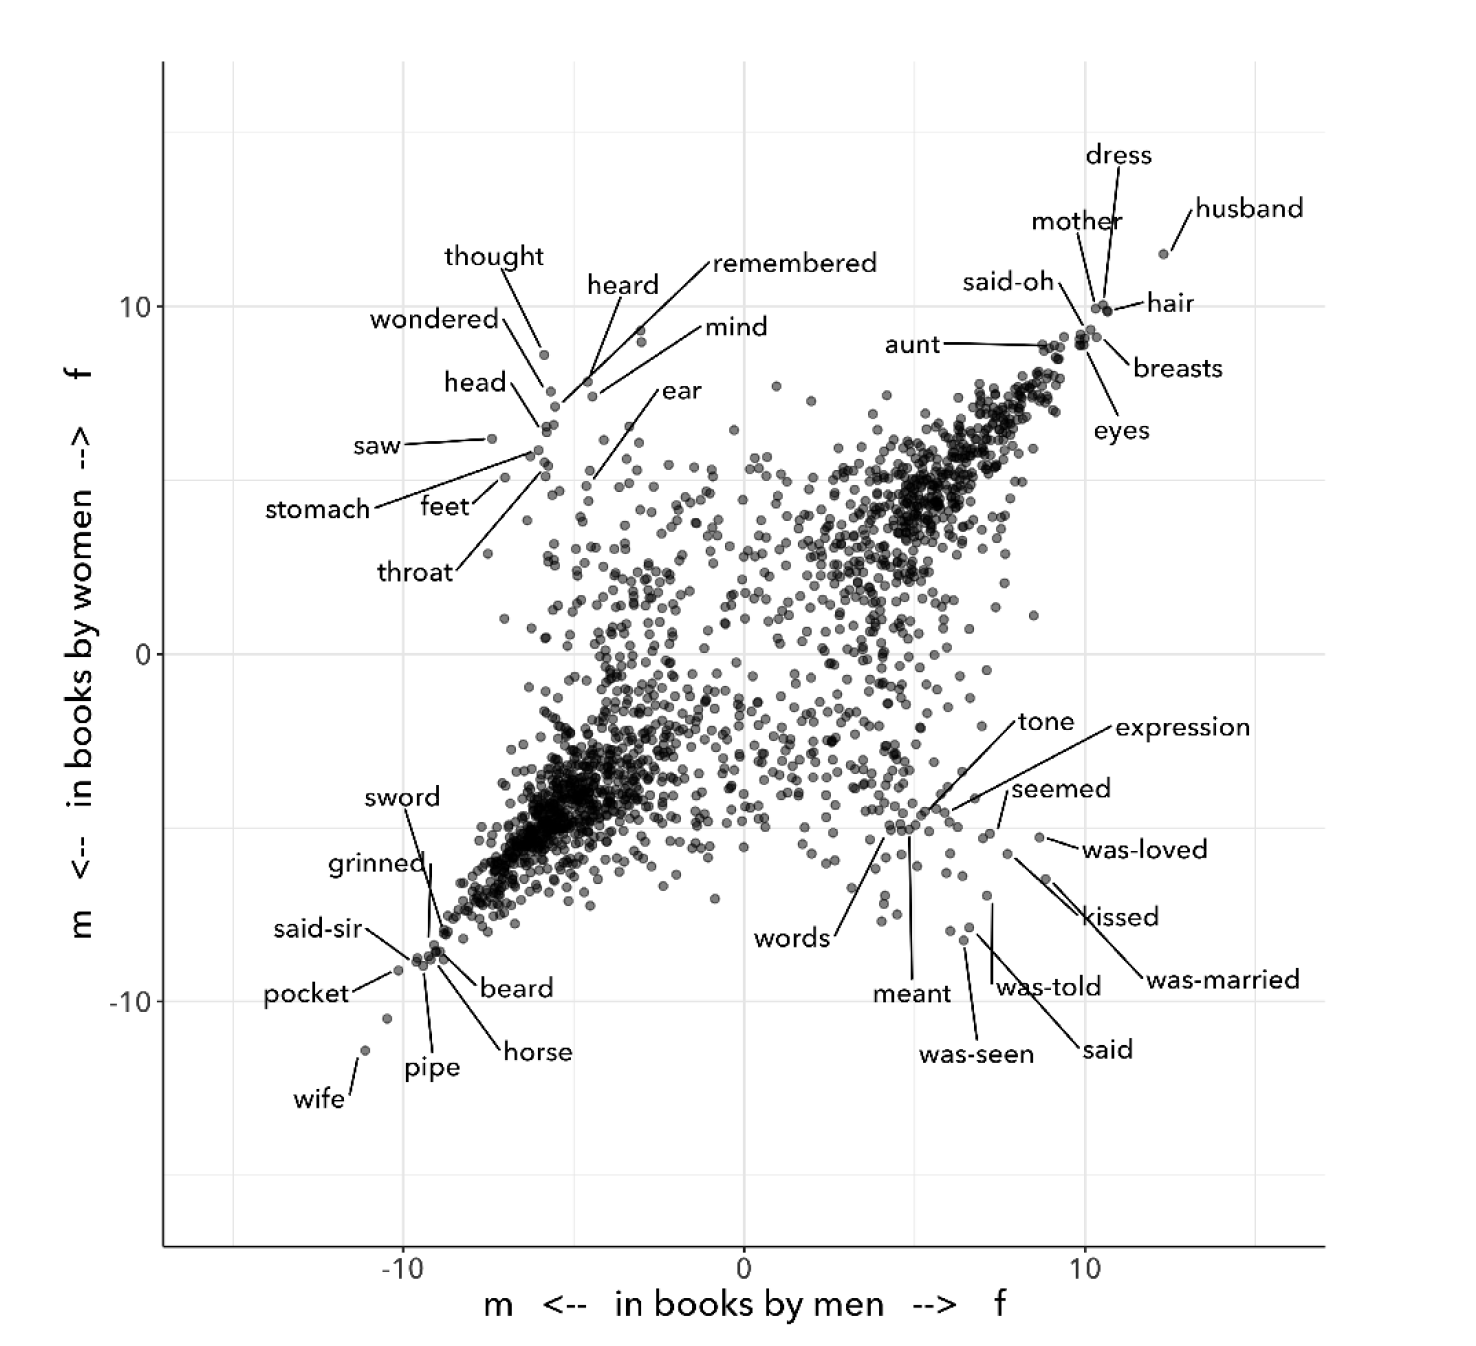
\includegraphics[width=.9\linewidth]{./img/Underwood.png}
\end{center}

Critiquing scholars like Underwood, Nan Z. Da argues that quantitative
methods are ill-suited for literary criticism. She accusses Underwood
and other distant reading practitioners for trading "speed for
accuracy, and coverage for nuance" (620). Of her many gripes with
quantitative methods, which include "technical problems, logical
fallacies," and a "fundamental mismatch betwen the statistical tools
that are used and the objects to which they are applied" (601), she
emphasizes the lack of reproducible results, the idea that one
researcher's process can be reproduced by another with identical
output, which is essential to statistical methodologies. She
demonstrates with an experiment of Topic Modelling, which is the
processing of large texts in order to generate a number of "topics"
within the corpus. Researchers often use Topic Modelling as a way of
speed-reading a massive corpus to get a sense of what it is about
without having to actually look at the text. Da attempts to verify the
results of a Topic Modelling experiment by replicating the process on
her own machine, a replication that fails. She concludes that, "if the
method were effective, someone with comparable training should be able
to use the same parameters to get basically the same results"
(628-629).\footnote{Da's emphasis on the “reproducible” in CLS extends Franco
Moretti's originating call for a “falsifiable criticism”: both
advocate for a methodology that is as reliable and verifiable as the
social sciences. According to Moretti: “Testing” literary
interpretations be the same process as in scientific disciplines --
demanding that interpretations are “coherent, univocal, and complete,”
and are tested against “data” that appears to contradict it (\emph{Signs}
21). (another quote: “The day criticism gives up its battle cry ‘it is
possible to interpret this element in the following way,’ to replace
it with the much more prosaic, ‘the following interpretation is
impossible for such and such a reason,’ it will have taken a huge step
forward on the road of methodological solidity” (\emph{Signs} 22).)} For Da, reproducibility of method is a benchmark for
reviewing and assessing the efficacy of quantification.

Despite their vastly different committments, scholars like Underwood
align with Da on the value that they place on reproducibility, which
is an ultimately conservative investment. Underwood demonstrates how
the critic reproduces their assumptions in the questions and data used
at the outset in a way that structures the final result. Da's emphasis
on the reproducible suggests that, to be useful, quantitative literary
criticism ought to resemble something more like statistical analysis:
if the method can be verified, can be copied and reproduced, then the
interpretive conditions might be universalized. 

\subsubsection{Drucker's skewing the graphs}
\label{sec:org7d36620}

Underwood and Da overlook the way that quantification can be used to
disrupt assumptions or reveal the constructed nature of data. In
contrast to Underwood and Da, Johanna Drucker is careful to dispell
the illusion of "raw data," which comes already reduced to fit
whatever parameters required by analysis. Because data always
undergoes a transformation in order to be quantified, its complexity
has already been compromised. As a result, Drucker argues,
quantification techniques such as visualizations in graphs and charts
inevitably misrepresent the data they are meant to convey. To
illustrate this process, Drucker presents a chart displaying the
amount of books published over several years. The chart appears to
convey production during this specific time period, but Drucker
explains that publication date is an arbitrary metric for capturing
production.\footnote{Drucker implicitly refers to the first chapter from Franco
Moretti's \emph{Graphs, Maps, Trees} (2007), throughout which Moretti
graphs novels by their publication date between 1700 and 2000 and
draws conclusions about the relationship between genre and generations
of readers.} She brings to the surface all the assumptions made
in such a metric, for example, the limitations of "novel" as a genre
and the connotations behind "published," which suggests date of
appearance, but has no indication of composition, editing, review,
distribution. Each piece of data carries with it the result of many
interpretive decisions, that carry with them varying degrees of
opacity, which are all necessary in order to present complex concepts
like book production as a bar on a chart. Drucker explains: "the
graphical presentation of supposedly self-evident
information\ldots{} conceals these complexities, and the interpretative
factors that bring the numerics into being, under a guise of graphical
legibility" (Drucker par. 23).

To resist the reductions of "data," a term that deceptively connotes
that which is "given," Drucker proposes thinking of data as "capta,"
which suggests that which is taken. Drucker's "capta" is deliberately
creative, turning graphical expressions into expressive metrics:
components used for measurement, like lines or bars on a graph, break,
blur, or bleed into one another. Objects are not discrete entities,
but interact with the other objects in the visualization. For example,
in a bar graph of book publications by year, she warps the graphical
metrics, making some of them fuzzy, wider, shorter, in an attempt to
show that publication as a metric elides other information such as
composition, editing, purchasing, etc.

\begin{center}
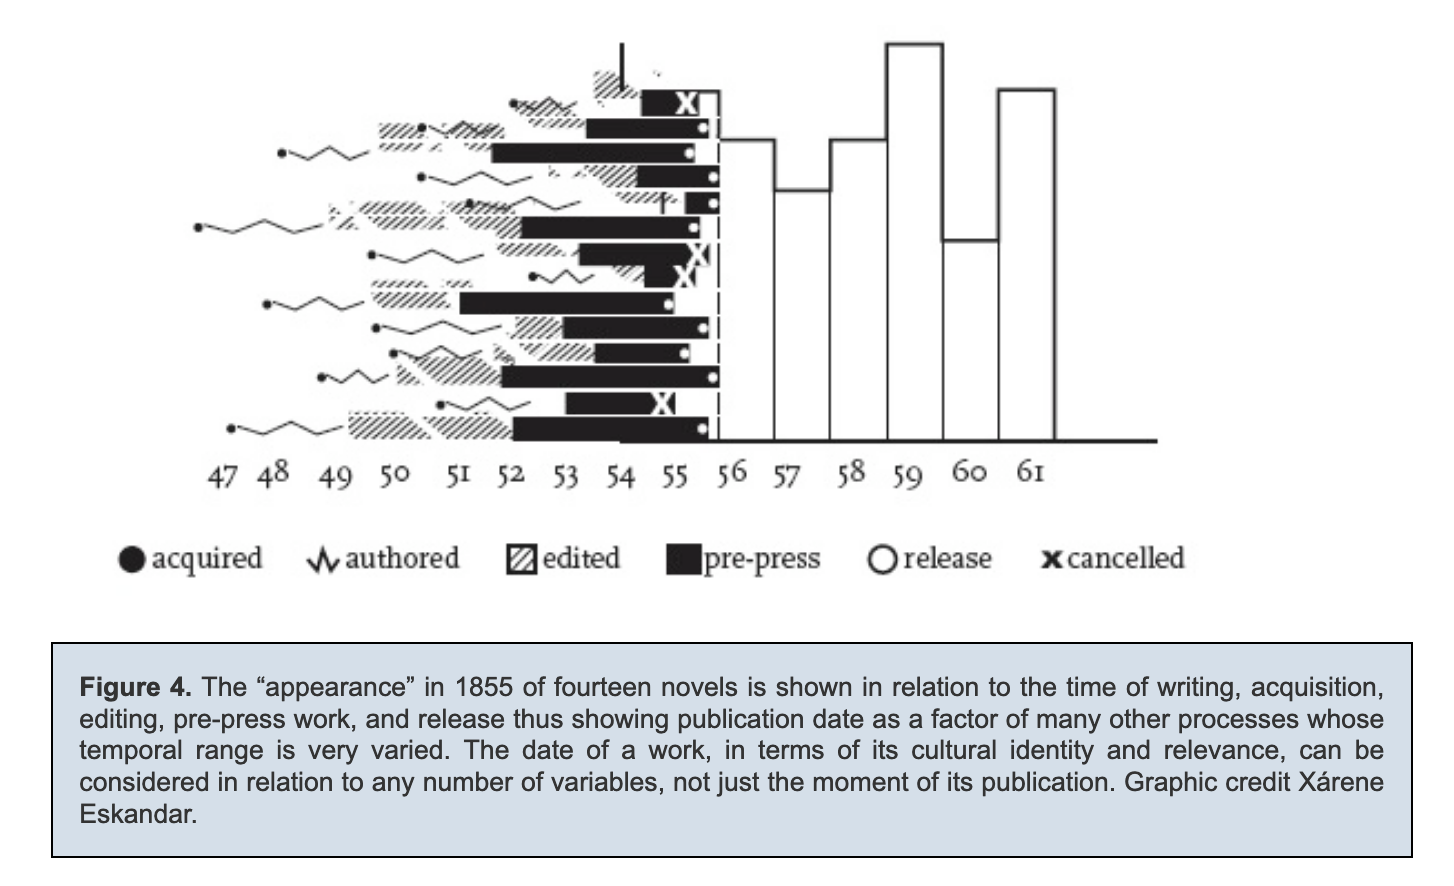
\includegraphics[width=.9\linewidth]{./img/Drucker.png}
\end{center}

Emphasizing "capta" is a way of figuring elements that have been
reduced, resolved, or ignored in traditional quantitative
analysis. Drucker makes evident what is overlooked or assumed when
dealing with complex subjects by muddling (rather than simplifying)
the relationship between elements.

\subsubsection{Mandell: deconstructing gender with computation}
\label{sec:org700084d}
Drucker points out how data that is taken (capta) can be rendered
graphically to sugesst the complexity of that data. Laura Mandell
similarly explores solutions for approaching the reduction of data,
particularly of gender, into what she calls the "M/F binary."\footnote{Mandell, Laura. “Gender and Cultural Analytics: Finding or
Making Stereotypes?” Debates in Digital Humanities 2019. Edited by
Matthew K. Gold and Lauren Klein. University of Minnesota Press, 2019.}
Mandell critiques recent uses of stylometery by Matthew Jockers and
Jan Rybicki, which analyze "masculine" or "feminine" modes of writing
by computing syntax, diction, and other linguistic features. Mandell
demonstrates how the M/F binary is reified "by presenting conclusions
about “male” and “female” modes of thinking and writing as if the M/F
terms were simple pointers to an unproblematic reality, transparently
referential and not discursively constituted" (par. 5). Mandell's
examination marshalls key findings from feminist theory, drawing from
Judith Butler, among others, to assert that gender is a socially
constituted category, a "performance" that can be historicized. She
illustrates the guiding power of the M/F binary in her critique of
Jockers and Rybicki, which find that they essentialize gender by
relying on stereotypes in their premises.

Rather than discount quantitative methods, however, Mandell suggests
that it can open up the way we deconstruct our understanding of
quantification and gender: "if we admit that categories such as gender
are being constructed both by the measurer and the measured\ldots{} we
might then be able to use stylometry to experiment with new taxonomies
of gender" (par. 37). To demonstrate how gender is "constructed," she
poses a counter experiment with genre, which finds that genre analysis
cuts across the gender binary. She comapres the stylistic qualities of
a female writer, Mary Wollenstonecraft, against two male writers,
William Godwin and Samuel Johnson, revealing that: "Wollstonecraft’s
sentimental anti-Jacobin novels most resemble Godwin’s sentimental
anti-Jacobin novels\ldots{} whereas her essays most resemble Johnson’s
writings" (par. 29). Wollenstonecraft's writing resembles both male
and female writing, depending on the genre. To analyze the highly
constructed category of "gender," then, one must also consider genre:
"separating gender from other markings (genre, era of composition) is
not possible: historical time and genre are not incidental to, but
constitutive of, gender" (par. 35).

The similarities between gender and genre, however, work to evacuate
how gender is \emph{constitutive} of the subject. She points out that both
are kinds of performance than can be learned: "features of both gender
and genre, while highly discernible, are also highly
imitable. (par. 30). Mandell asserts that "Anyone can adopt gendered
modes of behavior, just as anyone can write in genres stereotypically
labeled M/F" (par.30). Here, she takes Butler's points about gender
performativity beyond its purview: indeed, Butler's description of
performativity as a process, rather than a singular act, emphasizes
the lack of an autonomous subject that performs gender. In \emph{Bodies
that Matter}, her follow-up to \emph{Gender Trouble}, Butler explicitly
warns against the interpretation that gender is decided by the
subject, to be put on and off at will like clothing. Rather, according
to Butler, the subject \emph{is produced} by gender, which allows the
subject to emerge: "construction is neither a subject nor its act, but
a process of reiteration by which both 'subjects' and 'acts' come to
appear at all" (xviii). Crucially, Butler asserts that gender
\emph{precedes} and \emph{constitutes} the subject. This is not to say that
Mandell is wrong about gender being constructed, but that her
assumption, that "categories such as gender are being constructed both
by the measurer and the measured" misses an important point about the
autonomy of subject (par. 38). According to Butler, the subject only
emerges as an effect of gendered performance.

Even so, Mandell's work suggests further ways of drawing attention to
the complexity of gender, which harness the interactive affordances of
the computer. Her emphasis on visualization and movement inform how
one might "animate numerical processes rather than fixing their
results as stereotype" (par. 7). The dynamicity of computation, which
allows one to run data iteratively, feeding new inputs into new
results, complicates any straighforward understanding of the M/F
binary. Mandell explains that “Computer screens\ldots{} afford the fluid
exploration of parameters and taxonomies, through which many sorts of
experiments can be tested: interactive visualizations can give us not
objective answers rooted in aggressively reductive oppositions, but
parallax, multiple perspectives for viewing a very complex reality”
(par. 38). She points to programming and visualization tools to
emphasize how they might multiply our understanding of gender:

\begin{quote}
We could break the algorithm’s capacity to produce “a strong gender
signal” by simply increasing the number of gender categories to be
sorted. Experts in the field could create metadata to generate a
completely new taxonomy to replace the tired M/F binary: “men writing
as men,” “women writing as women, “women writing as men,” “men writing
as women,” “unspecified (anonymous) writing as men,” “unspecified
writing as women,” “men writing as men (byline) in the voice of a
woman (woman narrator),” “men writing as unspecified (anonymous
byline) in the voice of a woman,” “women writing as men (byline) in a
voice of unspecified,” etc.—whatever categories are presented by title
pages, prefaces, narrators’ discourses, and research into authorship
attribution found. par. 36
\end{quote}

Mandell points to manipulation of gender categories, which gives the
researcher more opportunities for input.

\subsubsection{So \& Roland: using machine to ignite human thinking}
\label{sec:org2379e1e}

One example of distant reading explores how computation might handle
questions of racial identity and discourse in novels. Richard Jean So
and Edwin Roland use machine learning to explore the constructedness
of social categories like race by experimenting with an algorithm that
evaluates authorship by race according to the vocabulary used by the
author.  When they look more closely into these results, they find
that the algorithm reveals different levels of variance in words
traditionally attributed to white and black authors. While novels by
white authors are distinguished by a low variance in this vocabulary,
novels by black authors show a greater variance in vocabulary
(66). They conclude that white authorship as a category only coheres
when it evaluates against the incoherence of black authorship. Put
simply, they find that whiteness as a category \emph{depends} on the
characterization of blackness.\footnote{Tie this relationship on the white/black binary to Eve
Sedgwick's points about binaries containing an oppostional dynamic in
which the subordinated term props up the dominant term.} They point out that, of course,
this process is useful not for what we learn about race but for what
we learn about the machine, particularly in the way that the results
reveal errors that open up areas for further analysis. They isolate
one text, James Baldwin's novel, \emph{Giovanni's Room} (1956), which was
wrongly categorized as being written by a white author. So and Roland
point out that this misclassification evokes a critical debate about
this text's elision of explicit references to race and sexuality,
whereby blackness is displaced in favor of an implicit whiteness that
serve to "cipher[s] identity" (69). The algorithm revealed six words
in \emph{Giovanni's Room} that influenced the categorization, one of them
in particular signals white authorship, the term "appalled." This term
only occurs once in the text, in the early scene where David (the
narrator) describes his relationship to his father. Here, David
regrets his friendliness which comes at the expense of his
fatherliness: "I did not want to be his buddy. I wanted to be his
son. What passed between us as masculine candor exhausted and appalled
me" (Rpt. in So and Roland 71). So and Roland's analysis emphasize the
connotations of whiteness in "appalled," which has the middle French
root, "apalir," meaning "to grow pale" (71). They insightfully
conclude that the word "appalled" in the text marks "the moment David
develops a troubled relationship to normative masculinity [as] also
the moment he becomes 'white'" (71). Their analysis thus contributes
to the ongoing debate about the imbrication between race and sexuality
in the novel.

In a sense, So and Roland are confronting the same problem as Da: what
to do with a case of computational error [which comes with attendant
assumptions about reproducibility\ldots{}]. But rather than write off
quantitative methods, So and Roland suggest an interesting way out of
the problem: use the error as a starting point for further
analysis. While "Race is a category that escapes measurement or simply
renders it untenable," the machine is an apt tool for studying this
category (60). They isolate the error as an opportunity to explore the
differences in the ways humans and machines might approach racial
identity. Because race is a social construct, and machines only impute
meaning that is encoded into them, than it stands to reason that
machines might be ideal instruments for studying the construction of
race. Thus they turn the central mismatch between data analysis, which
works to "identify and label objects," and minority discourse
analysis, which "critique[s] and problematize[s] the very idea of
categories," into a point for interrogation (63). In this case, the
algorithm offers an opportunity for understanding how whiteness as a
category depends on the contrast of blackness as "other." Quantifying
race reinforces differences, reductions, stratification, as “Reading
race distantly thus requires quantification of racial identity or
racialized language” (60). Looking more closely at the specific
results of this analysis, like the function of the term "appalled" in
\emph{Giovanni's Room}, they can make more daring leaps of speculation
about how whiteness, while displacing blackness, also gestures toward
a troubled understanding of gender and potentially, sexuality. So and
Roland assert that: "If the general class of the misclassified points
to the erosion of the machine's initial binary understanding of white
and black, a close analysis of a single misclassified text can reveal
what precisely motivates that ontological undoing" (68). Rather than
being "fundamentally mismatched," the machine and minority discourse
are particularly suited for one another, as the machine uses highly
constructed and reductive method that allows practitioners to
deconstruct social categories.

The example with "appalled" is totally idiosyncratic--the word occurs
once through the entire novel. But paying attention to error upends
the value of reproducibility. Because race is a construct, we must use
a "reflexive method that is able to identify its own elisions while
also pointing to new insights and opportunities for research”
(72). Roland and So's work combines a deconstructive with a
speculative methodology. They run a computation, look for an error,
and use that error as an opportunity to learn about the ways that
categories are constructed. They assert their goals: “To illustrate
the limits of standard computational methods for the analysis of race
and to produce a series of results that nonetheless advance our
understanding of the texts and authors under investigation… exposing
the racial limitations of computation can reveal things otherwise
occluded within literary history” (61). They are using computers in an
unintuitive way, computing for indeterminacy. While this work is
essential for bringing together quantitative and critical race
discourses, it also doesn't give enough credit to the ways that
\emph{computers}, in presenting formalized schemas of race, transform data
toward speculative ends. This is to suggest that perhaps a
deconstructive and specualtive methodology is too ambivalent. What if
we began with the notion of the appalled?  What if we looked further
into the way that race is generated by vocabulary?  Not in order to
further understand how race operates (computers will never be as
subtle thinkers as we are), but to direct human subtlety more attently
to computer output. What if, rather than using the machine to study
human constructs, we used the machine to spur human thinking?

\subsubsection{{\bfseries\sffamily WAITING} synthesis of Mandell and SoRoland}
\label{sec:orgace0e1d}
Both Mandell and SoRoland are using the machine to take apart these
categories of race and gender.
But let's look to the ways that the machine presents ever new
configurations of race and gender. Let's look at the form as a \emph{queer
form}. 
\begin{enumerate}
\item → What kind of knowledge are we trying to create? Aren't we now
\label{sec:org330045f}
operating as if it is possible to “distant read” in the first
place? That there are things which can be quantified, if only we
ask the right questions? When we look to the "occluded", are we
hunting or speculating?  The orientation we take toward our object
has an effect. Are we trying to recover or to speculate?
\end{enumerate}


\subsection{textual scholarship and deformance}
\label{sec:orgc9e4901}
how dh methods descendant from textual scholarship offer a model of
deformance that can incorporate key ideas from queer theory, like
citationality/resignification, to do distant reading.
\subsubsection{distant reading not to achieve scale, but for reconfiguration}
\label{sec:org76065a6}
According to Underwood, distant reading is less useful for studying a
single text in depth and more useful for taking a long view of larger
corpora. He sets up an opposition between computer and human reading:
"Computational analysis of a text is more flexible than it used to be,
but it is still quite crude compared to human reading; it helps mainly
with questions where evidence is simply too big to fit in a single
reader's memory" (xxi). He is right to point out that a computer
cannot (yet) draw inferences like a human can, and that a human cannot
"read" at the same speed as a computer. Yet, his emphasis on the
limitations of human memory suggests another way that that computers
can guide and enhance the human reading of smaller texts. What the
computer properly does is arrange a set of data--of any size--for
human consumption. This involves processing datasets into new forms
and configurations that can then be scrutinzed by a human
reader. Although Underwood uses distant reading to "to find a
perspective that makes\ldots{} scholars all congruent with each other,"
quantitative methods can supplement human memory by approaching
memory, specifically working memory, as a resource, rather than a
hindrance (\emph{Distant Horizons} 32). The computer can re-arrange text in
a way that focuses the attention span of the reader on elements
previously unseen or overlooked. Underwood's focus on
falsifiability--the idea that distant reading can process more
evidence to give a more "complete" picture--blocks out the ways that
the ways that quantitative literary analysis, or distant reading,
works in coordination with existing human capacities.
\subsubsection{Textual scholarship offers a new way of looking at text}
\label{sec:org6ff07be}
Now we shift our attention to a body of literary criticism that offers
another perspective for handling textual data. The field of textual
scholarship, and particularly the editorial practice of deformance,
opens up a way of thinking about data that is performative rather than
representative. Critics like Jerome McGann, Tanya Clement, and
Katherine Bode take an approach toward text that resists the
conservatism of traditional textual scholarship, which has generally
aimed for the recovery and preservation of the ideal text. Rather than
pursue recovery, these textual scholars explore new ways of reading
our textual inheritance that creates new possibilities for discovery
and speculation. Their methodology opens a space for key ideas in
queer theory about how to work within (and resist) the constraints of
language as a significatory system. This is about working within a
system to transcend the determining structure of that system.

\subsubsection{overview of textual scholarship}
\label{sec:orgf98778a}
To proceed, I will present a historical trajectory of editorial
practices that tells a story of textual scholarship. Textual
scholarship is the study, annotation, and editing of textual
materials, like manuscripts and books. Within textual scholarship,
textual criticism focuses specifically on identifying and analyzing
variants of manuscripts and books with the purpose of selecting an
ideal witness as the basis for a critical edition. As they further
idealize the value of authorial intention, theories of textual
criticism increasingly delimit the purpose and purview of the
editor. The history of textual criticism thus presents an arc, which
first tends toward I call the conservative or restorative and then,
with the advent of digital technology, the productive. With the
popularization of digital tools, editing becomes less about restoring
or correcting a text, and more about finding ways to open up the way
that a text is read and interpreted. My purpose here is to carve a
critique that emphasizes how the \emph{creative} capacity functions within
textual editing paradigm. My reading will therefore look to ways that
editorial pracitices have opened up a space for the editor's role as a
content creator rather than recoverer or preserver.

The conservatism of textual editing begins with Ronald B. McKerrow,
leading twentieth-century Shakespearean scholar. McKerrow proposed an
influential model for "copy-text" editing, which bases the text (the
"copy-text") on an early witness that most closely resembles the
author's original intention. The editor defers to this text for
editing, favoring the earliest copy-text to settle differences among
variants. However, this approach created its own resistance among
textual scholars, who decried the "the tyranny of the copy-text."
While maintaining reliance on an early copy-text for accidentals
elements like punctuation and spelling, the Greg-Bowers-Tanselle
method of textual criticsm empowers editors to judge between numerous
witnesses the text's more substantive elements\footnote{Greg, Walter W. "The Rationale of Copy-Text," \emph{Studies in
Bibliography}, Vol. 3, 1950/1951, pp. 19-36; Bowers, Fredson. \emph{Textual
and Literary Criticism}, 1959; Tanselle, Thomas. \emph{A Rationale of
Textual Criticism}, 1992.}. The resulting
critical edition is eclectic, drawing from multiple sources and
depending heavily on the editor's judgment to determine authorial
intention. Fredson Bowers and Thomas Tanselle advanced Walter
W. Greg's influential work, \emph{The Rationale of Copy-Text}, further
extending the importance of authorial intention and encouraging
editors to make careful and deliberate choices about substantive
elements. Tanselle, in particular, places much value in the editor who
is able to recongize and manage inevitable textual
corruption. According to Tanselle, the physical variant is a vessel
for the text, whose ideal form can only be realized by the editor. He
makes a distinction between "work" and "text":
\begin{quote}
Those who believe that they can analyze a literary work without
questioning the constitution of a particular written or oral text of
it are behaving as if the work were directly accessible on paper or in
sound waves\ldots{} [In fact,] its medium is neither visual nor
auditory. The medium of literature is the words (whether already
existent or newly created) of a language; and arrangements of words
according to the syntax of some language (along with such aids to
their interpretation as pauses or punctuation) can exist in the mind,
whether or not they are reported by voice or in writing. Tanselle
16-17
\end{quote}
Tanselle explains that physical act of inscription involves tools that
ultimately corrupt the pure ideas or intentions of the
writer. Therefore, every writer needs an editor that can help her
realize the ideal form of the text on paper. The editor, as someone
who is sufficiently distant from the creation and transcription of the
text, can objectively intimate its true intention. Therefore, the text
closest to the author’s intention is one scrupulously edited by a
textual scholar. Put another way, every author requires a thorough and
knowledgeable editor in order to most closely realize his intentions
on the page.

Toward the end of the 20th century, textual critics like Jerome McGann
and Donald F. McKenzie take another perspective on the effect of
inscription and tools on the textual material. McGann explores how
editorial practices, rather than aim for some ideal authorial version
of a text, might open up the ways that a text might be interpreted. He
builds off McKenzie's ideas about the influence of the social in
textual criticism. McKenzie's groundbreaking work, \emph{Bibliography and
the Sociology of Texts} (1999), studies how the materiality of texts,
includes sound and electronic media, takes on new forms and meanings
in in their reprinting and reproduction. McKenzie traces this
distribution, what he calls the "sociology" of texts, by examining the
social context that produced each witness, pointing out that "Every
society rewrites its past, every reader rewrites its texts, and if
they have any continuing life at all, at some point every printer
redesigns them” (25). Because the book is never a single object, but a
product of a number of human agencies and mechanical techniques that
are historically situated, no witness, regardless of scrupulous
editing by the critic, can represent an "ideal" version. McGann takes
these ideas and applies them to a digital editing environment, to
explore how electronic media might present the different variants of a
text. He explains that, because textual criticism in print format is
limited to linear and two dimensional form of the codex, this
criticism is limited to the same form as its object of
study. Paper-based editions, according to McGann’s experience, are
clunky and inadequate, and newer editions often “feed upon and develop
from [their] own blindness and incapacities” (McGann 2001, 81). By
contrast, digital editions can be designed for complex, reflexive, and
ongoing interactions between reader and text. Indeed, “[a]n edition is
conceivable that might undertake as an essential part of its work a
regular and disciplined analysis and critique of itself” (McGann 2001,
81). McGann explains that changing one’s view of the original
materials through the process of building the edition calls its
original purpose into question. McGann points out that his work on the
digital \emph{Rossetti Archive} brought him to repeatedly reconsider his
earlier conception and goals, asserting that the archive "seemed more
and more an instrument for imagining what we didn’t know” (2001,
82). 

Like books, digital media is also limited, but it holds potential for
the way it displays information. The technical experience of editing
electronic texts encourages the speculation on new potentialities
about its presentation. McGann introduces the term “quantum poetics”
to indicate the volatile potentiality for meaning contained in every
element of a literary text. He explains that, “Aesthetic space is
organized like quantum space, where the ‘identity’ of the elements
making up the space are perceived to shift and change, even reverse
themselves, when measures of attention move across discrete quantum
levels” (McGann 2001, 183). The meaning of particular words in a
literary text depends upon a multitude of factors, from antecedent
readings and pathways through that text, to the significance of
immanent elements such as typography and blank spaces, all of which
the reader can only process a limited amount. In its potentiality,
McGann asserts, “Every page, even a blank page\ldots{} is n-dimensional”
(2001, 184). Accordingly, digital tools could expose literature’s
inherent potentialities by carving new paths across familiar texts. In
this way, McGann argues for tools that facilitate tactile and
intuitive engagements of texts within an environment that opens itself
up to multiple dimensions of reading.

This radical potentiality of a text's quantum poetics is a result of
the limitation of digital media, which creates a tranformation upon
literary material into a new form. McGann's work thus takes the
limitations of computation--the fixing and disambiguation of data--and
turns it into a vehicle for analyzing literary material. He, along
with Lisa Samuels, describe literary interpretation as performance, or
what they call "deformance." Deformance works by estranging the reader
from her familiarity of the text, and relies on the the volitality of
meaning of particular words that depend upon a multitude of factors,
from antecedent readings and pathways through that text, to the
significance of immanent elements such as typography and blank spaces,
all of which the reader can only process a limited amount. A
"deformative criticism" therefore distorts, disorders, or re-assembles
literary texts to discover new insights about its formal significance
and meaning. McGann and Samuels offer the example of reading a poem
backward, where “the critical and interpretive question is not 'What
does the poem mean?' but 'How do we release or expose this poem’s
possibilities for meaning?'" (2001, 108).
\subsubsection{performative analysis with focus on apparatus}
\label{sec:orge99d134}

I now turn to the work of Katherine Bode and Tanya Clement, both of
whom have deep investments with traditions of textual scholarship,
particularly the scholarship of Jerome McGann, that has influenced
early experiments with digital humanities in English
departments. Although their approaches vary in their specific topics,
methods, and results, they are connected in an investment for, in the
words of McGann, "imagining what we don't know" (82).

Building off the humanistic approaches in textual scholarship and
bibliography, Bode reframes literary analysis as performative. Bode
incorporates insights from Karen Barad's feminist scientific
methodology to argue against representationalism, or "the idea that a
knowing human agent symbolically expresses – or represents – some
thing-in-the-world (that thing is unchanged by that expression, and
that expression is more available or apprehensible to the subject than
the thing itself) ("Data Beyond Representation" par. 2). Barad's work
intervenes in theoretical physics to argue how the researcher is
always implicated in the object of study, and she proposes a theory of
"agential realism," where objects in the world do not precede their
interaction, but rather, 'objects' emerge through particular
"intra-actions" (Barad 58). Bode brings Barad's point about the
assumption of representation from physics to computational modelling,
where she explains that "entities don’t pre-exist engagements but are
generated in an ongoing or emergent way, by those intra-actions"
("Data Beyond Represenation" par. 2). For Bode, what statisticians
value as “representativeness” or “reproducibility” isn’t as important
(within a humanities context) as the materiality of the
apparatus. Rather than attempt to secure a factual or objective status
of the data, we should double down on the material processes of using
our tools. Accordingly, Bode suggests that we approach literary
databases in performative terms, taking a self-conscious appraisal of
the tools of analysis, as "effects of material-semiotic engagements"
("Data Beyond Representation" par. 15).

In troubling the subject/object boundary, examining "how\ldots{} we
inscribe the boundaries we often presume to represent," Bode offers an
example with her current project, \emph{Reading at the Interface}, which
explores the ways that Australian literature has been characterized by
various "paratexts," or "writings about literature."  ("Data Beyond
Representation par 11.) The project explores paratexts across various
platforms, including academic journals, newspapers, \emph{Goodreads}, and
\emph{Librarything}, to see how they have represented the boundary of
"Australian Literature." Bode looks at how the process of data
collection makes a distinction between the main text and the
"paratext," or the metadata like title, author, and publication
information of the text. She is interested in how her inquiry
literally creates boundaries of what we understand to be "text" and
"paratext" in Australian literature. This activity indicates, for
Bode, how the researcher is intevening with the object of
analysis. Bode that she's "not interested in representing discussion
of “Australian literature” on Goodreads so much as in materialising
that platform in ways that cannot be separated from [her] categories
of analysis" ("Data Beyond Representation" par. 19). Her research
finds that an attention to the "apparatus," or the instrument of
analysis, is crucial in exploring the performative aspects of
inquiry. Drawing from a physics understanding, where "an apparatus is
a specific material configuration, including of physicists, wherein
certain properties become determinate, while others are excluded,"
Bode applies the figure of the apparatus to literary databases (Bode
"Data Beyond Representation, par. 24). Instead of looking at what is
being reproduced, she urges literary researchers to look at how human
engagement has entangled with and created the object of analysis.

\subsubsection{play leads to discovery}
\label{sec:org56b4051}

Tanya Clement's work with sound incorporates praxis, visualization,
embodiment, and play toward a theory of performantive criticism. She
uses figures and methods from audio analysis to reconsider the ways we
approach digitized text. In a project on text visualization, she puts
forth a theory of “play,” in which the critic "performs" the work,
much like the way that musicians interpret a musical score. She uses
the audio analysis tool "ProseVis" to visualize the prosodic elements
of Gertrude Stein's poetry, which creates dynamic spaces for the
reader to interact with the visualization. Using ProseVis, the reader
can navigate through the visualizations and manipulate the metrics for
analysis. Clement makes the analogy between musical scores and
quantitative visualizations to emphasize how both "create another
level of abstraction with which the interpreter engages" ("Distant
Listening par. 7). Clement points out that a musical score "is read,
but it is also meant to be played, to be spatialized in time and
embodied by voices (or instruments) within a certain physical and
hermeneutical context" ("Distant Listening" par. 10). She argues that
the same is true for visualizations of text: "One 'reads' a
visualization, but to 'play' the visualisation is to engage the
spatialized interpretation of that visualisation as an embodied reader
in a situated context within a specific hermeneutical framework
("Distant Listening" par. 10). The multiple levels of abstraction for
containing the "work" of the text multiply the levels of engagement
with that text. Clement's research takes this key finding from textual
scholarship and applies it to the critical process.

The unique affordance of digital environments, according to McGann,
Bode and Clement, is that they allow for numerable interventions upon
the textual object. Like a musical score, which "point[s] toward many
possible interpretive 'results' or readings," visualizaions can
provide a starting ground for different pathways of analysis ("Distant
Listening" par. 12). Human attention spans, rather than represent the
hurdle for computational methods to overcome, offer an opportunity for
re-imagining analysis as a process of deforming what we pay attention
to. The emphasis shifts from viewing text as something stable and
self-evident to something dynamic and subject to different
readings. As McGann speculates, engaging with texts on a computer
could be as intimate a process as engaging with them on paper. We
might use digital tools as “prosthetic extension of that demand for
critical reflection,” with which the reader is able to feel her way
through the text (18).


\subsection{{\bfseries\sffamily IN\_PROGRESS} queer performance \& citationality}
\label{sec:org4252835}
\subsubsection{overview}
\label{sec:orgdaefe70}
Distant reading can evolve by borrowing from key findings from queer
theory that allow it to embrace the performative/productive aspects of
quantification. In particular, Butler's idea of gender performativity
coheres with deformative reading. Butler describes performativity as a
repetative activity, constrained by regulatory norms, which produces
subjects. Although performativity regulates subjects toward
heteronormative practices, it can also be coopted into subversion. In
the process of repetition, subjects have the possibility of
resignifying meaning by producing it differently. This resignification
allows subjects to work within their limitations to resist dominant
structures while maintaining their own sense of exclusion without
being coopted. In other words, they can be in the system but not of
the system.

\subsubsection{Butler}
\label{sec:orgf7a29f2}

\begin{enumerate}
\item Butler's theory of performativity:
\label{sec:org4f42e2c}

In her groundbreaking book, \emph{Gender Trouble: Feminism and the
Subversion of Identity} (1990), Judith Butler famously disrupts
contemporary feminist theorizations about sex and gender; namely, that
sex is biological while gender is constructed; and that the gender, as
a construction, is an expression of the subject. According to Butler,
there is no such thing as a stable gender identity, or even a subject
that exists prior to gender expression. Rather, Butler argues that
gender is a performance--a series of repeated acts by which the
subject, in the ongoing enactment of gender expression according to
heteronormative regulatory schemas, emerges. Major criticism of this
work resists the idea that both sex and gender are discursively
produced, insisting upon the physicality of the sexed body as a basis
of identity. In \emph{Bodies That Matter} (1995), Butler responds to this
criticism by delineating the process of performativity, where what is
experienced as the physical body, its boundaries and its sexuality,
only materialize through the repetition or “citation” of cultural
norms. Her concept of "citation" emphasizes the iterability of the
performative practice, whereby each action "cites" or implicitly
signals an authorizing norm. According to Butler, performance consists
of this habit of citation, the ongoing process of submitting behavior
to a regulatory norm. Butler makes the general argument that body’s
materiality is discursive, that the “sexed body” is a residue or
"sentimentation" that emerges from the signification and
re-signification of whatever social power or understanding about sex.

In \emph{Bodies that Matter}, Butler's central concern is to explore how
language and the body engage. She approaches this concern by
identifying the issue with representation: "Can language simply refer
to materiality, or is language also the very condition under which
materiality may be said to appear?" (6). Specifically, Butler wonders
whether language can indicate a body that has not yet been imbued with
meaning, a body "prior to signification" (6). She finds that language
cannot--for to refer to the body, language must first posit that body,
and in the positing, it assumes meaning. Therefore, the signification
of the body actually creates the body: "This signification produces as
an \emph{effect} of its own procedure the very body that it nevertheless
and simultaneously claims to discover as that which \emph{precedes} its own
action" (6). Butler thus claims that language only works to \emph{produce}
signification, rather than reflect a prior reality:
\begin{quote}
If the body signified as prior to signification is an effect of
signification, then the mimetic or representational status of
language, which claims that signs follow bodies as their necessary
mirrors, is not mimetic at all. On the contrary, it is productive,
constitutive, one might even argue performative, inasmuch as this
signifying act delimits and contours the body that it then claims to
find prior to any and all signification. Butler 6
\end{quote}
Language cannot simply point to a reality. Rather, language actually
produces that reality. The effect is that, in the process of citation,
which is the ongoing re-signification that appeals to regulatory
norms, subjects cannot speak outside the powers that structure
speech. Subjects are always interpellated by a discourse prior to
their citing it. However, in finding that the body cannot exist prior
to signification, Butler isolates a productive quality of language,
which will be central to the ways that language offers a way out of
the significatory circle.

\item The solution: resignification
\label{sec:orgc8e705f}

Butler then insists that resignification of these citations is the way
out of this significatory circle.

Amid this regulatory structure, however, lies the possibility of
resignifying sex/gender though subversive practices. Butler offers an
example in the resignification of the “queer,” which has been
transformed from a term of abjection to one of empowerment.

The central problem of being stuck in performance is also the
solution. Butler takes on language as something that can be
productive, that can resignify meaning. It is the option available to
those who are trapped within the signification system.

\begin{itemize}
\item We cannot speak outside the powers that structure speech. Because
sex is always constructed, because we are constructed through sex,
we can never get out of the signifying system. Subjects are always
interpellated by the discourse prior to citing it. Like protocol,
discourse determines all connections; in gender, the subject only
comes into intelligibility through the matrix of gender. The only
freedom that is possible resides within this power of discourse,
resignifying it, perhaps through parody or impersonation. The
abject, through disidentification has the ability to resignify
against the logic of the norm.
\item The performance of resignification is a political act: “What would
it mean to cite a law to produce it differently?”
\begin{itemize}
\item We see this in the word “queer” which has been
re-appropriated---something thatsignified abjectness now means
defiance. We can also use repetitionto re-signify
identification, to the point where it loses itspower. In Paris
is Burning, not only are the male drag performersexposing the
superficiality of gender, but also performing care in away that
is feminine, “mothering” “housing” “rearing” each other.
\item “The compulsion to repeat an injury is not necessarily the
compulsion to repeat the injury in the same way or to stay fully
within the traumatic orbit of that injury. The force of repetition
in language may be the paradoxical condition by which a certain
agency---not linked to a fiction of the ego as master of
circumstance---is derived from the impossibility of choice…. Paris
is Burning might be understood as repetitions of hegemonic forms of
power that fail to repeat loyally and, in that failure, open
possibilities for resignifying the terms of violation against their
violating aims” (383).
\end{itemize}
\end{itemize}

Butler takes on language as something that can be productive, that can
resignify meaning. It is the option available to those who are trapped
within the signification system. 

\begin{itemize}
\item language is not mimetic, representative, rather, it is productive:
\begin{itemize}
\item "If the body signified as prior to signifiation is an effect of
signification, then the mimetic or representational status of
language, which claims that signs follow bodies as their
necessary mirrors, is not mimetic at all. On the contrary, it is
productive, constitutive, one might even argue performative,
inasmuch as this signifying act delimits and contours the body
that it then claims to find prior to any and all signifcation"
(6).
\end{itemize}
\end{itemize}


\item representing the irrepresentable: something missing that is an
\label{sec:orgfb9d974}
enabling constraint 

Luce Irigaray's task is to show how the feminine has been excluded
from philosophy. She is critiquing the writings by Plato on the
form/matter and body/soul distinction.
\begin{itemize}
\item "Irigaray's task\ldots{}. is to show that those binary oppositions are
formulated through the exclusion of a field of disruptive
possibilities. Her speculative thesis is that those binaries, even
in their reconciled mode, are part of a phallogocentric economy that
produces the “feminine” as its constitutive outside" (10).
\item "The economy that claims to include the feminine as the subordinate
term in a binary opposition of masculine/feminine excludes the
feminine, produces the feminine as that which must be excluded for
that economy to operate" (10).
\end{itemize}

"For how can one read a text for what does \emph{not} appear within its own
terms, but which nevertheless constitutes the illegible conditions of
its own legibility? (p. 11)\ldots{} One cannot interpret the philosophical
relation to the feminine through the figures that philosophy provides,
but, rather, she argues, through siting the feminine as the
unspeakable condition of figuration, as that which, in fact, can never
be figured within the terms of philosophy proper, but whose exclusion
from that propriety is its enabling condition" (p. 12).

"she mimes philosophy—-as well as psychoanalysis—-and, in the mime,
takes on a language that effectively cannot belong to her\ldots{}  This
contestation of propriety and property is precisely the option open to
the feminine when it has been constituted as an excluded impropriety,
as the improper, the propertyless" (12).

"Irigaray’s response to this exclusion of the feminine from the
economy of representation\ldots{} I’ll show you what this unintelligible
receptacle can do to your system; I will not be a poor copy in your
system, but I will resemble you nevertheless by miming the textual
passages through which you construct your system and showing that what
cannot enter it is already inside it (as its necessary outside), and I
will mime and repeat the gestures of your operation until this
emergence of the outside within the system calls into question its
systematic closure and its pretension to be self-grounding\ldots{}.In this
sense, she performs a repetition and displacement of the phallic
economy. /This is citation, not as enslavement or simple reiteration
of the original, but as an insubordination that appears to take place
within the very terms of the original, and which calls into question
the power of origination that Plato appears to claim for himself./ Her
miming has the effect of repeating the origin only to displace that
origin as an origin" (18).

--> this process applies aptly to distant reading. Reading for
enabling structures. The difference is that we aren't valorizing scale
or speed reading; rather, we are reading for that which is hidden,
surpressed, which determines that which is visible.


\item Butler looks toward the horizon, where queerness can never be
\label{sec:org447e280}
defined, but remains outside the known. The goal is not to be
inclusive, it's to preserve this space without being coopted.

\begin{itemize}
\item "The task is to refigure this necessary “outside” as a future
horizon, one in which the violence of exclusion is perpetually
in the process of being overcome. But of equal importance is the
preservation of the outside, the site where discourse meets its
limits, where the opacity of what is not included in a given
regime of truth acts as a disruptive site of linguistic
impropriety and unrepresentability, illuminating the violent and
contingent boundaries of that normative regime precisely through
the inability of that regime to represent that which might pose
a fundamental threat to its continuity. In this sense, \textbf{radical
and inclusive representability is not precisely the goal}: to
include, to speak as, to bring in every marginal and excluded
position within a given discourse is to claim that a singular
discourse meets its limits nowhere, that it can and will
domesticate all signs of difference. If there is a violence
necessary to the language of politics, then the risk of that
violation might well be followed by another in which we begin,
without ending, without mastering, to own—-and yet never fully
to own—-the exclusions by which we proceed." (25).
\end{itemize}



\item Synthesis between Butler's and Bode's performance
\label{sec:org344b0f3}

The next step is to show how paying attention to the assumptions of
data (simplicity, reproducibility) relates to queer deconstruction,
embodiment, performance, speculation, as described by queer
critics. 

a parallelism between Bode and Butler: 
"When computational literary scholars engage with literary phenomena,
I'm suggesting that we have two options. So we can approach this
practice in representationalist terms. We can imagine that our
databases and data sets and models are symbolic expressions by knowing
agents us have stable self evident and self contained objects that
exist elsewhere. And that actually follow a print based model of how
literature exists. Alternatively, we can understand our databases or
models as part of the ongoing materialisation of literary texts as
emerging events always arising from an altering how the literary
pastas reconfigured" ("Computational Modeling: From Data Representation
to Performative Materiality")
\end{enumerate}



\subsection{{\bfseries\sffamily WAITING} Queer Distant Reading}
\label{sec:org269abb2}
\subsubsection{performance emphasizes materiality, movement, discovery}
\label{sec:org2f273a2}
In the section on reproducibility, I discuss how Underwood's analysis
on gender differences reproduces his assumptions about gender dynamics
as oppositional, as he readily admits: "this chapter has discovered
stable 'structural positions' only because it explores gender, for the
most part, as a binary opposition" (\emph{Distant Horizons} 140). The
question then becomes, how can we move beyond reproducing assumptions
in our analysis? The answer is to shift the objective of analysis from
the the reproducible to the alternative. The first value that this
reading method proposes is that of \emph{performance}. This value points to
the active qualities of critical analysis, emphasizing materiality and
sensitivity, movement and discovery. When reading is performative, the
process is more important than the product. 
\subsubsection{parallels between performance and deformance.}
\label{sec:org8fdf2aa}
\begin{enumerate}
\item the similarities between \textbf{performance} and \textbf{deformance},
\label{sec:orge3abad9}

\begin{itemize}
\item both are a process of deconstruction, resignification. Language
(like data) can be a productive force, rather than a mimetic
represenation of something prior, which produces the body.

\begin{itemize}
\item language is not mimetic, representative, rather, it is productive:
\begin{itemize}
\item "If the body signified as prior to signifiation is an effect of
signification, then the mimetic or representational status of
language, which claims that signs follow bodies as their
necessary mirrors, is not mimetic at all. On the contrary, it is
productive, constitutive, one might even argue performative,
inasmuch as this signifying act delimits and contours the body
that it then claims to find prior to any and all signifcation"
(6).
\end{itemize}
\end{itemize}
\end{itemize}

\item Distant reading is a way of reading that which is hidden,repressed, yet structures and determines that which is visible.
\label{sec:orgd73f39e}
\end{enumerate}

\subsubsection{Klein? Gaboury?}
\label{sec:orgec393d3}

\subsubsection{playing with voyant}
\label{sec:orgcc4b209}
I'm playing around with voyant tools on Giovanni's Room, and realizing
that my movements are carefully guided by this impression from textual
scholarship of deformance. At every step I am deforming the text,
creating a new text, with new potentials for reading. 

This deformance is an iterative process. 

What if we read only the sentences with the word "don't" in them?
There's a dip in the word "don't" toward the end of the novel, in
section 9. But when we get get the contexts into its own text
submission, there's a rise in this same sector. What's going on? 

Turns out, there's a spike in "don't"s in the middle of chapter five,
a spike that is surrounded with a dearth of don'ts. This explains why
there's a dip in the graph on the general text, and an uptick in the
graph that isolates don'ts from the general text.

This activity calls for closer attention to the area of the spike, and
its surroundings.

ag


\section{Move to other chapters}
\label{sec:org2ef6088}
\subsubsection{Altschuler and Weimar on reproducibility}
\label{sec:org01156dc}

--> reproducing something perfectly overlooks the ways that all
digital objects are unique, differentiated. Theory of textual
criticism which shows how ther are more interesting things to do then
create a digital "copy texte". 

This notion extends to digital humanist practitioners. 

they call to overturn the "unproblematic translatability of
information between the senses" while maintaining that reproduction is
the highest value. They argue to "texture the humanities", pointing
out that much of DH prioritizes the visual over other senses --
"privilege sight as the sense through which knowledge is accessible"
(74). Rightly so, they argue, “The textured DH we call for here
acknowledges that we cannot study knowledge only abstractly, apart
from the senses, and that we cannot study literature, art, and history
without including the history of embodied experiences” (74-75).
\begin{itemize}
\item “Touch This Page! uses 3-D printed facsimiles of raised-letter text
to inspire reflection on the assumptions most people make about
which senses are involved in reading” (82).
\end{itemize}

But they elide the one interesting trajectory when they place
reproduction over remediation/deformance. They state their aims: “to
expand the sensory accessibility of archives for all users and to do
so through the digital reproduction---rather than the translation---of
tactile knowledge” (76). Case example of the perfect reproduction:
\begin{itemize}
\item A scenario where “users\ldots{} can download a visual copy with
\end{itemize}
descriptive data, engage with the text in virtual reality, and create
their own textured facsimile. This technology once more makes possible
the tactile reading experiences for which this volume was designed and
promises library patrons a richer engagement with touch than most
archives can currently provide---even in person (85-86). 

The use case scenario makes the assumption that a reproduction is the
ideal form of textuality, despite their asserted aims for "diversity
of embodied experiences":
\begin{itemize}
\item “we must avoid tilting after the fiction of some ideal digital
surrogate---like a virtual reality system that would flawlessly
mimic original objects---lest we become digital Pierre Menards,
expending extensive energy to improve our reproductions to discover,
at last, that only the original perfects represents itself… Instead,
we envision in our tactile futures multiple strategies that could
not only open up access to varied experiences---past and
present---but also diversity the ways embodied experiences structure
our digital worlds” (86).
\item in order to open up “multiple strategies” and diversity embodied
experiences, we need a theory of text that is capacious enough to
accept variation and transmediation.
\item This argument overlooks deformance is a solution: the ways that
creating new texts, paratexts, creates new objects of knowledge. It
overlooks the performative, ala McGann, Clement.
\end{itemize}

In this view, digital becomes a means of optimization, efficiency,
total knowledge and understanding.

\subsubsection{The debates about TEI illustrates this tension between the}
\label{sec:orge15036d}
“conservative” and the “creative” impulses in textual editing, and
shows how an encoding method that is highly structured can be used to
mark or explore moments of textual instability or ambiguity.

\section{commands}
\label{sec:org4eeddc3}
c-c c-x f => create a new footnote
c-u c-c c-x f then select s => renumber footnotes

block quotes: \#+BEGIN\(_{\text{QUOTE}}\) \& \#+END\(_{\text{QUOTE}}\)

\section{annotated bib}
\label{sec:org02a663e}
\subsubsection{Moretti, Franco. Graphs, Maps, Trees: Abstract Models for Literary}
\label{sec:org420b810}
History. 2007.

This monograph defines and demonstrates “distant reading”, a deliberate abstraction and visualization of textual, bibliographic, and historical data about literature in order to answer questions about form and history of literature as a whole. 

\subsubsection{Drucker, Johanna. "Introduction," SpecLab: Digital Aesthetics and}
\label{sec:org98757a9}
Projects in Speculative Computing. 2009.

From a series of literary experiments at SpecLab at UVA, Drucker
posits a method of speculative computing that pushes against ideology
of mathesis---the idea that formal logic can represent or unlock human
thought and experience, that knowledge is information---by using
computational methods to provoke and push against what we think we
know.

\subsubsection{Ramsay, Stephen. Reading Machines: Toward an Algorithmic}
\label{sec:orgbd7e823}
Criticism. 2011.

Ramsay proposes a method of Algorithmic Criticism, which approaches
the constraints of computation as a liberating force that allows the
critic to reflect on her own phenomenal experience of texts rather
than seek definitive answers.

\subsubsection{Drucker, Johanna. "Humanities Approaches to Graphical Display." DHQ:}
\label{sec:org0f2cc72}
Digital Humanities Quarterly. 2011.

Digital Humanities needs graphical expressions that question, resist,
and reveal the assumptions of graphical display---that it is
observer-independent, objective, universal representations of
knowledge, that data is “raw” rather than captured.

\subsubsection{Felski, Rita. The Limits of Critique. 2015.}
\label{sec:org330890d}

Examines the role of affect in literary criticism, showing how the
hermeneutics of suspicion, as a militant mode of reading, forecloses
the possibilities of connection between reader and text.  

\subsubsection{Piper, Andrew. Enumerations: Data and Literary Study. 2018.}
\label{sec:org94d74c3}

Mixes distant and close reading in order to interrogate how the study
of literary quantity can lead to insights about literature.

\subsubsection{Landow, George. Hypertext 3.0: Critical Theory and New Media in an Era}
\label{sec:org165acc8}
of Globalization, 2006. Print.

The hypertext format engages the postmodern
(structuralist/post-structuralist and deconstructive) theories about
the multiplicity and instability of meaning in texts, as well as new
radical conceptions of authorship

\subsubsection{Fisher, Caitlin. These Waves of Girls, 2001. Web.}
\label{sec:org719ccba}

The profusion of hyperlinks frustrates the reader by offering too many
narrative paths. The reader’s frustration in navigating through the
hypertext relates to the work’s theme of sexual discovery. In
following the narrator as she develops her sexuality, the reader
experiences her own cycles of desire and frustration.

\subsubsection{Tenen, Dennis. Plain Text: the Poetics of Computation, 2017. Epub.}
\label{sec:orgb8b0049}

Tenen proposes a microanalysis, computational poetics, or an
archaeology of platforms and infrastructures (behind surface
content). We don’t engage directly with the textual conduit, so we
need to perform a media archaeology in order to have access to these
processes and be in charge of them.

\subsubsection{Rockwell, Geoffrey and Stefan Sinclair. Voyant-Tools. 2018.}
\label{sec:org93b86f0}

The par excellence example of literary criticism, which encourages
discovery.

\subsubsection{Galloway, Alexander. Protocol: How Control Exists after}
\label{sec:org46be7a2}
Decentralization. 2004.

Horizontal freedom requires universalization,
standardization. Resistance comes from within the system, using
exploits.

\subsubsection{Chun, Wendy. Control and Freedom: Power and Paranoia in the Age of}
\label{sec:orgf96a956}
Fiber Optics. 2006.

The potential for individual empowerment comes from harnessing our own
vulnerabilities and exposure. Without exposure, give and take, there
is no network.

\subsubsection{Bennett, Jane. Vibrant Matter: A Political Ecology of Things. 2010.}
\label{sec:orga2f358b}

Approaches the network as a vital non-anthropocentric ecology,
connecting humans to inert matter, endowing them with agency.

\subsubsection{Moten, Fred and Stefano Harney. The Undercommons: Fugitive Planning \&}
\label{sec:org88ec4f0}
Black Study. 2013.

A way of being in but not of the university, system,
network. Studying, collecting debt, being shipped are ways of relating
to one another that resists the system.

\subsubsection{Tufekci, Zeynep. Twitter and Tear Gas: the Power and Fragility of}
\label{sec:orgc33d6aa}
Networked Protest. 2017.

How humans aided with technology create networks, and how these
operate on the ground. What capacities do they have, how does their
horizontalism both help and hurt?

\subsubsection{Gaboury, Jacob. "Becoming NULL: Queer Relations in the Excluded}
\label{sec:orga37fc1b}
Middle." Women \& Performance: a Journal of Feminist
Theory. 28:2, 2018. pp. 143-158. Web.

What are queer modes of being within technological systems, modes that
refuse the gesture of capture and extraction? The NULL marker in SQL
offers a way of becoming that enacts a queer logic that is explicitly
situated within the logic of information systems but refuses this
gesture of capture and extraction.

\subsubsection{Kittler, Friedrich. Gramophone, Film, Typewriter. 1999.}
\label{sec:org213822f}

At first, media passes through symbols (written signifier), then
analog media is stored as physical traces, and now, new media loses
its specificity as a stream of numbers (“eyewash”), surface effects
which are then reassembled in the human. The human perceptual system
disperses into the apparatus.

What sense perceptions are we not aware of or not tapping? This opens
up the potentials of bits and fiber.

\subsubsection{Hayles, N. Katherine. Writing Machines. 2002.}
\label{sec:org16f6f6c}
Media is re-conceived, written, mediated for different formats---the
concept of remediation.

Reading technotexts takes place within a distributed cognitive
environment. We are part of a larger cybernetic circuit.

\subsubsection{Kirschenbaum, Matthew. Mechanisms: New Media and the Forensic}
\label{sec:org1b09deb}
Imagination. 2008.

Digital media create an illusion of immateriality---screen
essentialism. We should approach materiality on two levels, the formal
and forensic, to counter misunderstandings and occlusions of new
media. Electronic texts are not ephemeral or homogenous, they are
inscribed and made of unique traces.

\subsubsection{Blanchette, Jean-François, "A Material History of Bits." Journal of}
\label{sec:org4a68282}
the American Society for Information Science and Technology. No. 62:
pp. 1042-1057, 2011.

\subsubsection{Hansen, Mark. Feed-Forward: On The Future of 21st Century Media. 2014.}
\label{sec:org22f4e93}

The way that media works in the 21st century both marginalizes and
expands human perception. Things we have no awareness of are out there
feeling for us. We have an expanded perceptual reach, but our
sensations are indirect. This puts consciousness in an anticipatory
mode, always future oriented, focusing on what is nearly emergent---
“feed forward”.

\subsubsection{Woolf, Virginia, Emily McGinn, Amy Leggette, Matthew Hannah, and Paul}
\label{sec:orgc21ff86}
Bellew. "Comparing Marks: A Versioning Edition of Virginia Woolf's
'The Mark on the Wall.'" Scholarly Editing: The Annual of the
Association for Documentary Editing. Vol. 35, 2014.

Presents a “versioning edition” of the various print witnesses of
Woolf’s short story, the Mark on the Wall, from 1917-1944.  The
versioning edition’s attention to the story over time also implicitly
draws attention to the way that time functions on the level of
narrative.

\subsubsection{Peters, John Durham. The Marvelous Clouds: Toward a Philosophy of}
\label{sec:org29288aa}
Elemental Media. 2016.

\subsubsection{McKenzie, D.F. Bibliography and the Sociology of Texts. 1986.}
\label{sec:orgbef077b}

Individual texts are witnesses of an ideal text that is never to be
fully realized---the florid branches of an invisible trunk.
Bibliography is about tracking the book’s history as a social
document, the social relations involved in its transmission, and about
recognizing different critic’s “misreadings”. Book history is a
history of misreadings.

\subsubsection{Tanselle, Thomas. "A Rationale of Textual Criticism." 1992.}
\label{sec:orgad29351}

Texts are corrupted in physical form and require assistance of an
editor to present in an authentic state. The imperative of textual
criticism is to restore and correct.

\subsubsection{Derrida, Jacques. “Archive Fever: A Freudian Impression.”}
\label{sec:orgc5820ea}
Diacritics. Vol. 25, no. 2. 1995.

The archive works against itself: creating an archive also creates the
potential to forget and destroy. Externalization.  The instant of
archivization involves technology: ‘the prosthetic experience of the
technical substrate’ (22).

\subsubsection{McGann, Jerome. Radiant Textuality: Literature after the World Wide}
\label{sec:orga43a0e2}
Web. 2001.

Electronic editing ought to capture what is inherently n-dimensional
about literary texts---to engage in the quantum poetics of each
textual detail.

\subsubsection{Singer, Kate. “Digital Close Reading: TEI for Teaching Poetic}
\label{sec:org7938b78}
Vocabularies.” The Journal of Interactive Technology and Pedagogy. 3,
May 15, 2013.

Using TEI to teach close reading finds that one can approach it to
engage individualized readings---marking moments of textual
instability rather than formal aspects. Given that the tool is
flexible enough, we do not have to agree on a schema, standardize a
schema, in order to use the tool to engage the incommensurable.


\subsubsection{Caughie, Emily Datskou and Rebecca Parker. “Storm Clouds on the}
\label{sec:org30ad327}
Horizon: Feminist Ontologies and the Problem of Gender.” Feminist
Modernist Studies. 1:3, 230-242. 2018.

What do we do when our tools won’t allow us to capture or convey
certain elements of the text? It turns out that the limitations of the
computer are actually a good indicator of things that maybe should be
left unresolved or unfixed---like gender ontology.
\end{document}
